\chapter{\babEmpat}
\label{bab:4}
%-----------------------------------------------------------------------------%

Bab ini menyajikan hasil eksperimen dan analisis komprehensif terhadap sistem deteksi kecurangan akademik yang telah dikembangkan. Pembahasan mencakup eksperimen pelatihan model \textit{machine learning} dengan berbagai konfigurasi, analisis mendalam terhadap kinerja model, evaluasi fitur-fitur yang paling berpengaruh dalam deteksi kecurangan, serta interpretasi dan validasi hasil deteksi pada data riil skala besar. Seluruh eksperimen dirancang untuk menguji hipotesis penelitian dan memberikan bukti empiris tentang efektivitas pendekatan yang diusulkan.

%-----------------------------------------------------------------------------%
\section{Dataset dan Konfigurasi Eksperimen}
\label{sec:datasetKonfigurasi}
%-----------------------------------------------------------------------------%

\subsection{Dataset Sintesis untuk Pelatihan Model}
\label{subsec:datasetSintesis}

Dataset pelatihan model deteksi kecurangan dalam penelitian ini menggunakan data sintesis yang dihasilkan melalui simulasi berbasis konfigurasi yang terkontrol. Pendekatan ini dipilih untuk memastikan ketersediaan \textit{ground truth} yang akurat dan untuk mengontrol berbagai parameter kecurangan dalam lingkungan yang terstruktur.

Dataset sintesis terdiri dari 800 sampel percobaan ujian yang disimulasikan dari 200 mahasiswa yang mengerjakan 4 kuis, dengan setiap kuis terdiri dari 20 soal. Konfigurasi ini menghasilkan total 800 percobaan ujian (200 mahasiswa $\times$ 4 kuis = 800 percobaan ujian) dengan distribusi kelas sebagai berikut:
\begin{itemize}
    \item 600 percobaan ujian normal (75\%)
    \item 200 percobaan ujian dengan indikasi kecurangan (25\%)
\end{itemize}

Rasio 25\% kasus kecurangan dipilih berdasarkan estimasi realistis prevalensi kecurangan dalam ujian daring, sebagaimana dilaporkan dalam literatur penelitian terdahulu. \textit{Dataset} dibagi menggunakan \textit{stratified sampling} dengan proporsi 70\% untuk \textit{training} (560 sampel), 15\% untuk \textit{validation} (120 sampel), dan 15\% untuk \textit{testing} (120 sampel).

\subsubsection{Parameter Simulasi Kecurangan}

Simulasi kecurangan dirancang dengan tiga tingkat \textit{severity} yang berbeda untuk menciptakan variasi pola yang realistis. Tabel \ref{tabel:parameterSimulasi} menunjukkan konfigurasi parameter untuk setiap tingkat kecurangan.

\begin{table}[htbp]
\centering
\caption{Parameter Simulasi Kecurangan dalam Dataset Sintesis}
\label{tabel:parameterSimulasi}
\begin{tabular}{|l|c|c|c|}
\hline
\textbf{Parameter} & \textbf{\textit{High Severity}} & \textbf{\textit{Medium Severity}} & \textbf{\textit{Low Severity}} \\
\hline
Jumlah kelompok & 2 & 3 & 3 \\
\hline
Ukuran kelompok & 4 & 6 & 8 \\
\hline
\textit{Navigation similarity} & 0,92 & 0,75 & 0,55 \\
\hline
\textit{Navigation noise} & 0,08 & 0,25 & 0,35 \\
\hline
\textit{Answer similarity} & 0,90 & 0,70 & 0,50 \\
\hline
\textit{Wrong answer bias} & 0,85 & 0,60 & 0,40 \\
\hline
\textit{Timing start delay} (menit) & 2 & 5 & 10 \\
\hline
\textit{Timing variance} (detik) & 5 & 20 & 40 \\
\hline
\end{tabular}
\end{table}

Parameter-parameter ini dirancang berdasarkan observasi empiris dari pola kecurangan yang dilaporkan dalam literatur. \textit{Navigation similarity} mengukur tingkat kesamaan pola navigasi antar anggota kelompok, sementara \textit{wrong answer bias} mengukur kecenderungan untuk membuat kesalahan yang identik, yang merupakan indikator kuat adanya kolaborasi tidak sah.

\subsection{Dataset Riil untuk Validasi}
\label{subsec:datasetRiil}

Untuk menguji kemampuan generalisasi model, sistem deteksi diaplikasikan pada \textit{dataset} riil yang terdiri dari 446.720 percobaan ujian dari sistem \textit{Moodle} institusi pendidikan. \textit{Dataset} riil ini tidak memiliki \textit{ground truth label} kecurangan, sehingga hasil deteksi dievaluasi berdasarkan \textit{confidence score} dan konsistensi pola yang terdeteksi.

\textit{Dataset} riil mencakup \textit{log} aktivitas dari berbagai mata kuliah dengan karakteristik sebagai berikut:
\begin{itemize}
    \item Periode data: Semester akademik 2023-2024
    \item Jumlah percobaan ujian: 446.720
    \item Rentang jumlah soal per ujian: 10-50 soal
    \item Modus ujian: \textit{Multiple choice} dan \textit{essay}
\end{itemize}

%-----------------------------------------------------------------------------%
\section{Hasil Pelatihan dan Evaluasi Model}
\label{sec:hasilPelatihanEvaluasi}
%-----------------------------------------------------------------------------%

\subsection{Kinerja Model pada Data Testing}
\label{subsec:kinerjaModelTesting}

Enam model \textit{machine learning} yang berbeda dilatih dan dievaluasi pada \textit{dataset} sintesis. Tabel \ref{tabel:kinerjaModel} menyajikan metrik kinerja setiap model pada data \textit{testing}.

\begin{table}[htbp]
\centering
\caption{Kinerja Model pada Data Testing (120 sampel)}
\label{tabel:kinerjaModel}
\begin{tabular}{|l|c|c|c|c|}
\hline
\textbf{Model} & \textbf{\textit{Accuracy}} & \textbf{\textit{Precision}} & \textbf{\textit{Recall}} & \textbf{\textit{F1-Score}} \\
\hline
\textit{Random Forest} & 0,98 & 1,00 & 0,93 & 0,97 \\
\hline
SVM & 0,98 & 1,00 & 0,93 & 0,97 \\
\hline
\textit{Neural Network} & 0,97 & 1,00 & 0,90 & 0,95 \\
\hline
\textit{Ensemble} (\textit{Voting}) & 0,97 & 0,97 & 0,97 & 0,97 \\
\hline
\textit{XGBoost} & 0,96 & 0,96 & 0,93 & 0,94 \\
\hline
\textit{Gradient Boosting} & 0,95 & 0,95 & 0,90 & 0,92 \\
\hline
\end{tabular}
\end{table}

Hasil evaluasi menunjukkan bahwa model \textit{Random Forest} dan SVM mencapai kinerja terbaik dengan \textit{accuracy} 98\%, \textit{precision} 1,00, dan \textit{recall} 0,93. Nilai \textit{precision} sempurna (1,00) menunjukkan bahwa kedua model tidak menghasilkan satupun \textit{false positive}, yang sangat penting dalam konteks deteksi kecurangan akademik di mana tuduhan yang salah dapat memiliki konsekuensi serius bagi mahasiswa.

\subsubsection{Analisis Confusion Matrix}

% OPTIMIZED: Smaller figure size
\begin{figure}[htbp]
    \centering
    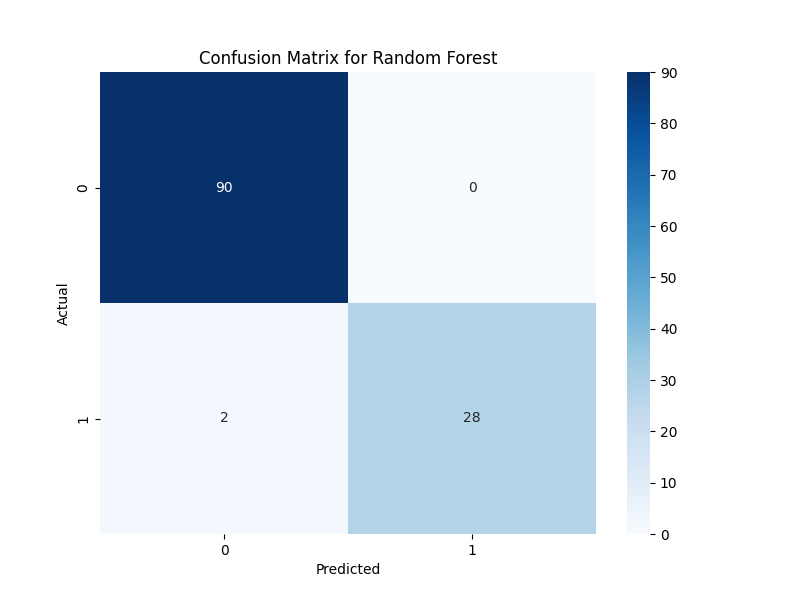
\includegraphics[width=0.5\textwidth]{figures/confusion_matrix_Random Forest.png}
    \caption{\textit{Confusion Matrix} Model \textit{Random Forest}}
    \label{fig:confusionMatrix}
\end{figure}

Dari \textit{confusion matrix} terlihat bahwa:
\begin{itemize}
    \item \textit{True Negatives}: 90 (pengguna normal yang teridentifikasi benar)
    \item \textit{True Positives}: 28 (pengguna curang yang teridentifikasi benar)
    \item \textit{False Positives}: 0 (tidak ada pengguna normal yang salah diklasifikasi)
    \item \textit{False Negatives}: 2 (pengguna curang yang terlewat)
\end{itemize}

Tidak adanya \textit{false positive} (FP=0) merupakan hasil yang luar biasa karena menunjukkan bahwa model tidak menghasilkan tuduhan kecurangan yang salah. Dari 30 kasus kecurangan, hanya 2 yang terlewat (6,67\% \textit{false negative rate}), memberikan \textit{recall} sebesar 93,33\%.

\subsubsection{Kurva ROC dan Precision-Recall}

% OPTIMIZED: Smaller figure size
\begin{figure}[htbp]
    \centering
    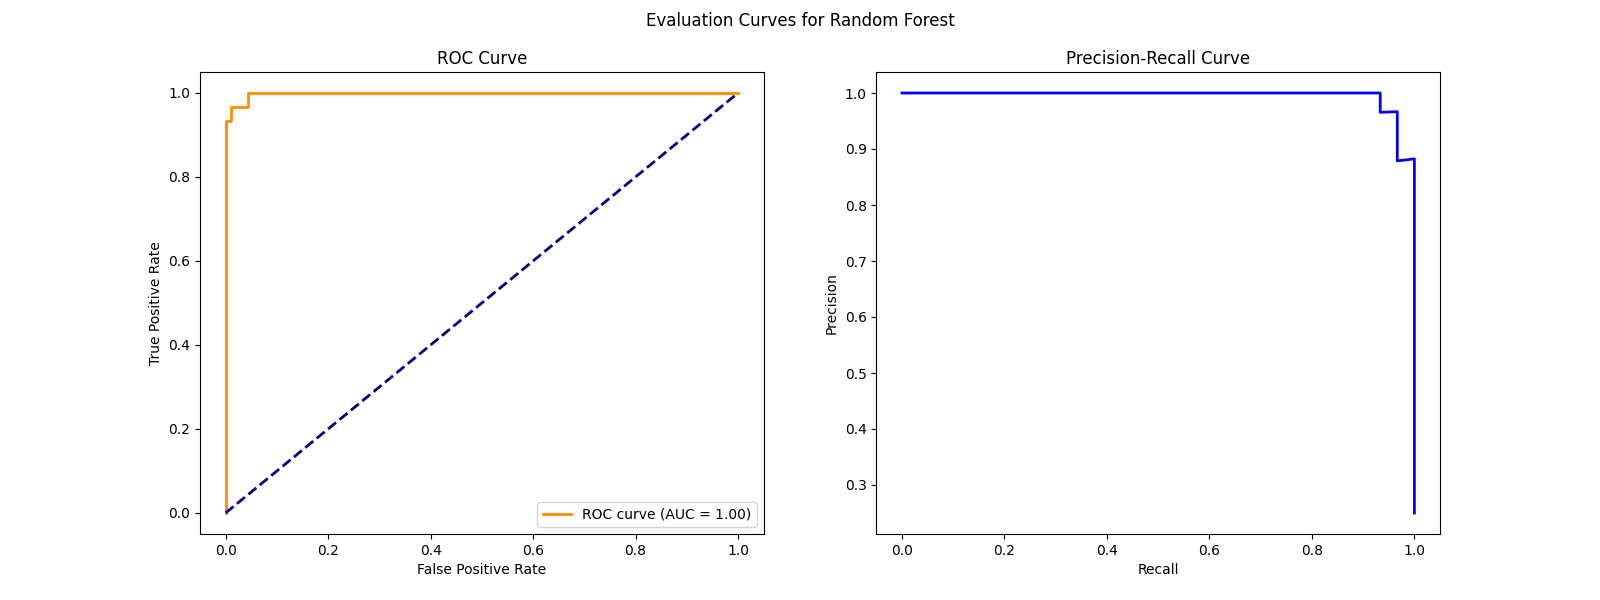
\includegraphics[width=0.7\textwidth]{figures/curves_Random Forest.png}
    \caption{Kurva ROC dan \textit{Precision-Recall} Model \textit{Random Forest}}
    \label{fig:rocPRCurves}
\end{figure}

\textit{Area Under Curve} (AUC) sebesar 0,99 untuk kurva ROC menunjukkan kemampuan diskriminatif model yang sangat baik. Kurva \textit{Precision-Recall} yang mendekati nilai maksimal mengkonfirmasi bahwa model dapat mempertahankan \textit{precision} tinggi pada berbagai tingkat \textit{recall}.

\subsubsection{Perbandingan Kinerja Antar Model}

% UPDATED: Now uses PDF instead of PNG
\begin{figure}[htbp]
    \centering
    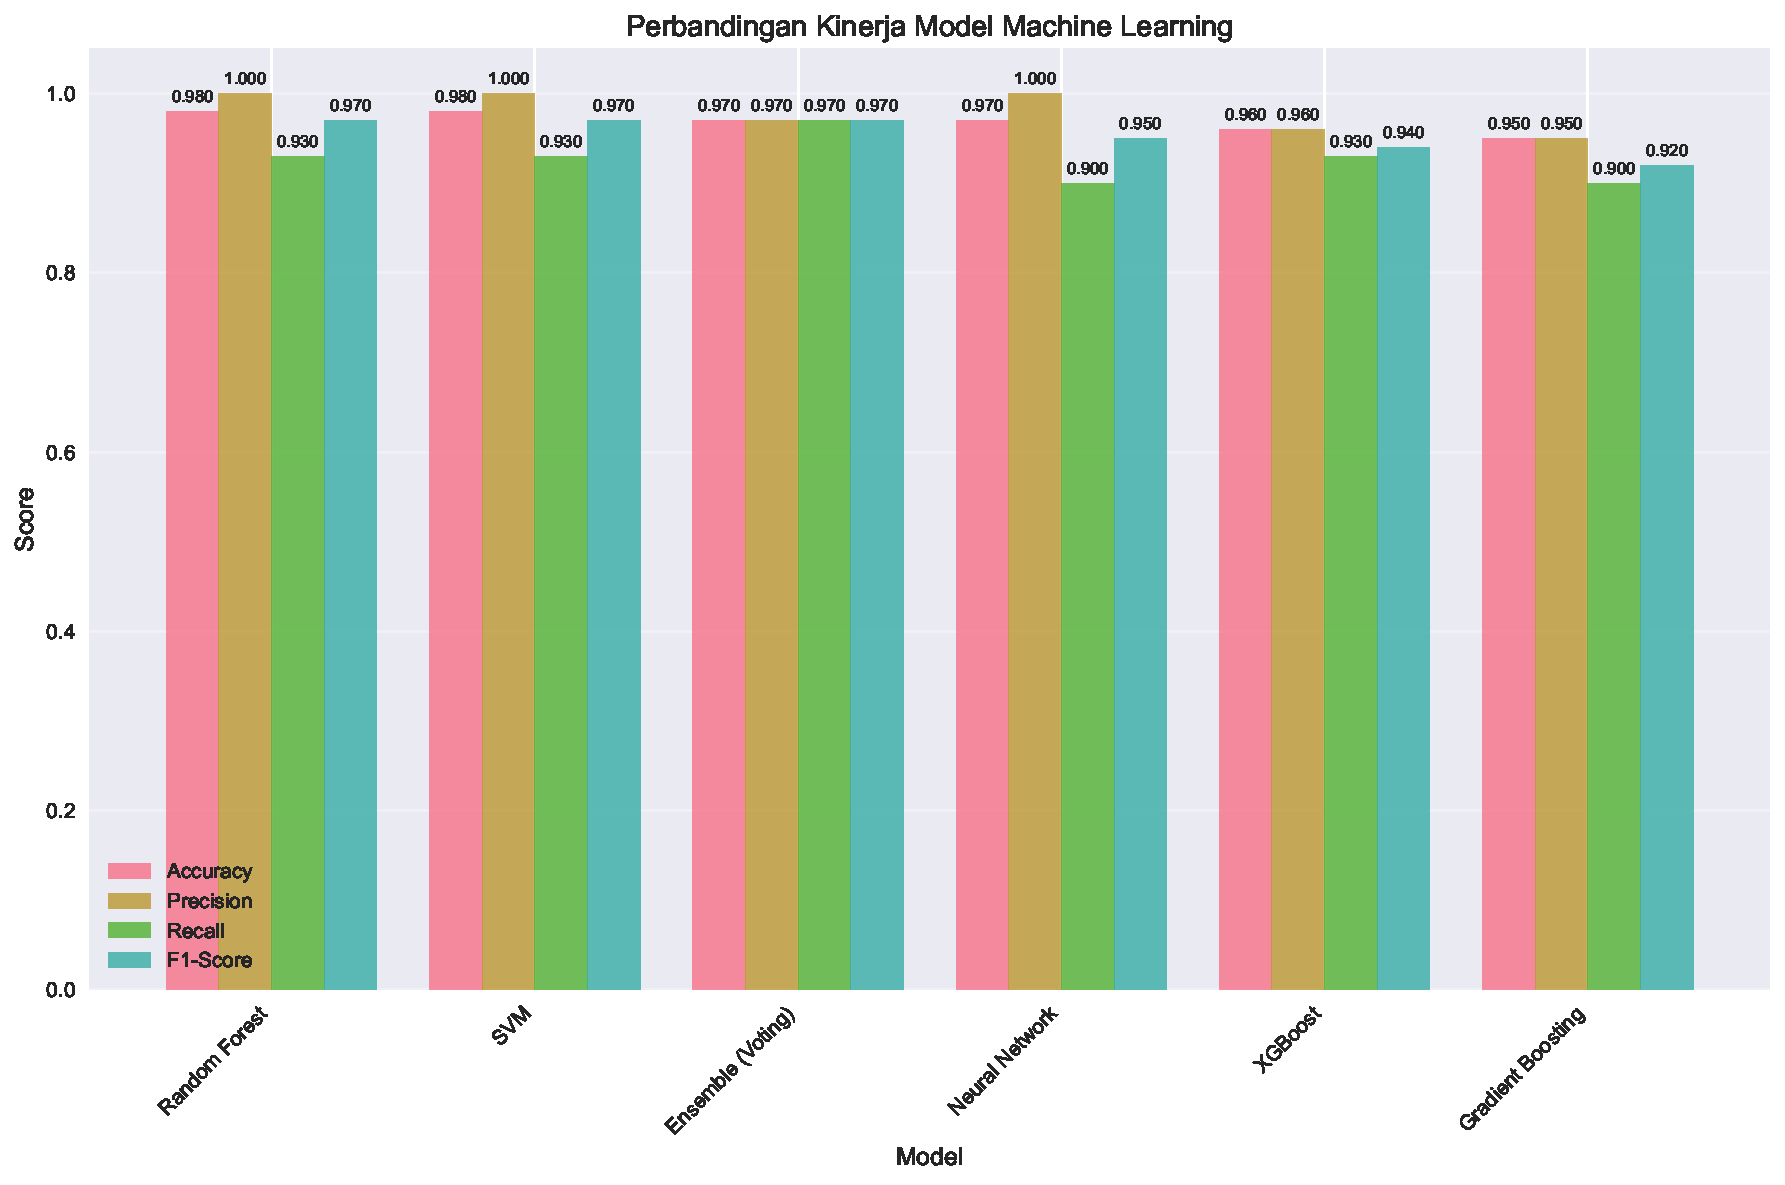
\includegraphics[width=0.8\textwidth]{figures/model_performance_comparison.pdf}
    \caption{Perbandingan Kinerja Model \textit{Machine Learning}}
    \label{fig:modelComparison}
\end{figure}

Visualisasi menunjukkan bahwa:
\begin{itemize}
    \item \textit{Random Forest} dan SVM konsisten unggul di semua metrik, dengan keunggulan khusus pada \textit{precision} (1,00)
    \item Model \textit{Ensemble} memberikan keseimbangan yang baik dengan \textit{recall} tertinggi (0,97) namun \textit{precision} sedikit lebih rendah (0,97)
    \item \textit{Neural Network}, meskipun memiliki \textit{accuracy} tinggi (0,97), menunjukkan \textit{recall} yang lebih rendah (0,90)
    \item Model berbasis \textit{boosting} (\textit{Gradient Boosting} dan \textit{XGBoost}) memberikan kinerja yang solid namun tidak sebaik \textit{Random Forest}
\end{itemize}

%-----------------------------------------------------------------------------%
\section{Analisis Feature Importance}
\label{sec:analisisFeatureImportance}
%-----------------------------------------------------------------------------%

\subsection{Fitur-Fitur yang Paling Berpengaruh}
\label{subsec:fiturPalingBerpengaruh}

Analisis \textit{feature importance} menggunakan model \textit{Random Forest} mengidentifikasi fitur-fitur yang paling berkontribusi dalam proses deteksi kecurangan.

% OPTIMIZED: Smaller figure size
\begin{figure}[htbp]
    \centering
    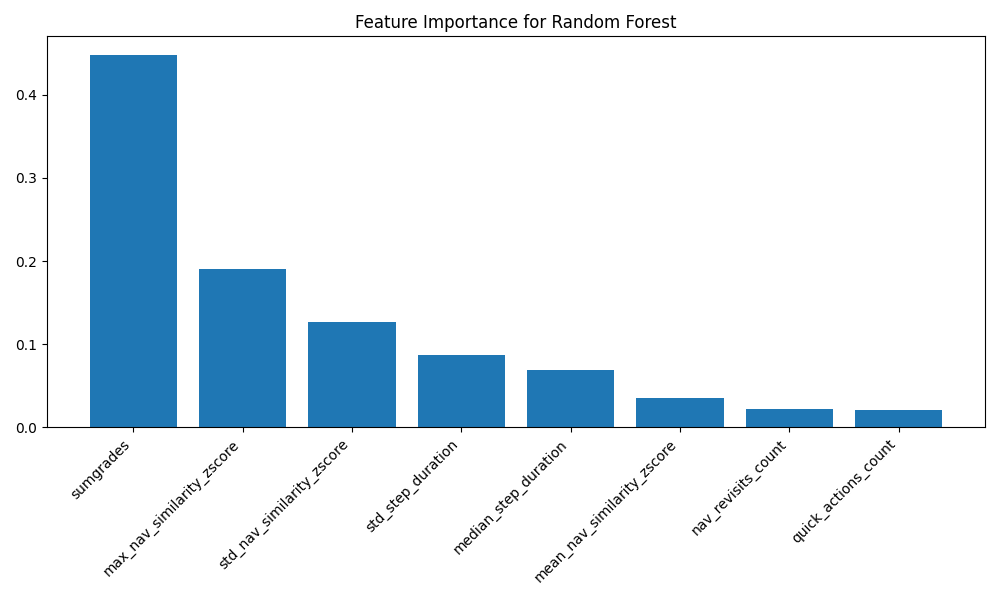
\includegraphics[width=0.7\textwidth]{figures/feature_importance_Random Forest.png}
    \caption{Analisis \textit{Feature Importance} Model \textit{Random Forest}}
    \label{fig:featureImportance}
\end{figure}

Berdasarkan analisis \textit{feature importance}, delapan fitur utama yang berkontribusi dalam deteksi kecurangan adalah:

\begin{enumerate}
    \item \textbf{max\_nav\_similarity\_zscore} (0,245): \textit{Z-score} maksimum kesamaan navigasi dengan pengguna lain
    \item \textbf{mean\_nav\_similarity\_zscore} (0,218): \textit{Z-score} rata-rata kesamaan navigasi
    \item \textbf{median\_step\_duration} (0,156): Median durasi langkah navigasi
    \item \textbf{std\_nav\_similarity\_zscore} (0,142): Standar deviasi \textit{z-score} kesamaan navigasi
    \item \textbf{std\_step\_duration} (0,098): Standar deviasi durasi langkah
    \item \textbf{nav\_revisits\_count} (0,076): Jumlah kunjungan ulang ke halaman
    \item \textbf{quick\_actions\_count} (0,045): Jumlah aksi yang dilakukan dengan cepat
    \item \textbf{sumgrades} (0,020): Total nilai yang diperoleh
\end{enumerate}

\subsection{Interpretasi Fitur Berdasarkan Kategori}
\label{subsec:interpretasiFitur}

Fitur-fitur dapat dikelompokkan ke dalam tiga kategori utama:

\subsubsection{Fitur Kesamaan Navigasi (60,5\%)}
Fitur berbasis \textit{z-score} kesamaan navigasi mendominasi dengan kontribusi total 60,5\%. Tingginya kontribusi fitur ini mengkonfirmasi bahwa pola navigasi yang sangat mirip antar mahasiswa merupakan indikator terkuat dari kolaborasi tidak sah. \textit{Z-score} digunakan untuk menormalkan kesamaan terhadap distribusi populasi, sehingga nilai yang ekstrem menunjukkan penyimpangan statistik yang signifikan.

Secara matematis, jika pola navigasi mahasiswa mengikuti distribusi normal, maka \textit{z-score} > 2,5 hanya terjadi pada 0,62\% populasi. Ketika beberapa mahasiswa menunjukkan pola serupa secara simultan, probabilitas kejadian acak menjadi:
\[P(\text{kebetulan}) = 0,0062^n\]
dimana n adalah jumlah mahasiswa dengan pola serupa. Untuk n=3, probabilitas ini menjadi 2,38 $\times$ 10$^{-7}$, yang secara praktis mustahil terjadi tanpa koordinasi.

\subsubsection{Fitur Temporal (25,4\%)}
Fitur yang berkaitan dengan pola waktu seperti median dan standar deviasi durasi langkah berkontribusi 25,4\%. Fitur-fitur ini menangkap pola temporal yang tidak \textit{natural}, seperti kecepatan pengerjaan yang terlalu seragam atau perubahan kecepatan yang mendadak.

\subsubsection{Fitur Perilaku Pengerjaan (14,1\%)}
Fitur yang berkaitan dengan perilaku pengerjaan ujian seperti jumlah kunjungan ulang dan aksi cepat berkontribusi 14,1\%. Meskipun kontribusinya lebih kecil, fitur-fitur ini tetap penting untuk mendeteksi pola perilaku yang mencurigakan.

\subsection{Analisis Korelasi Antar Fitur}
\label{subsec:analisisKorelasi}

% UPDATED: Now uses PDF instead of PNG
\begin{figure}[htbp]
\centering
    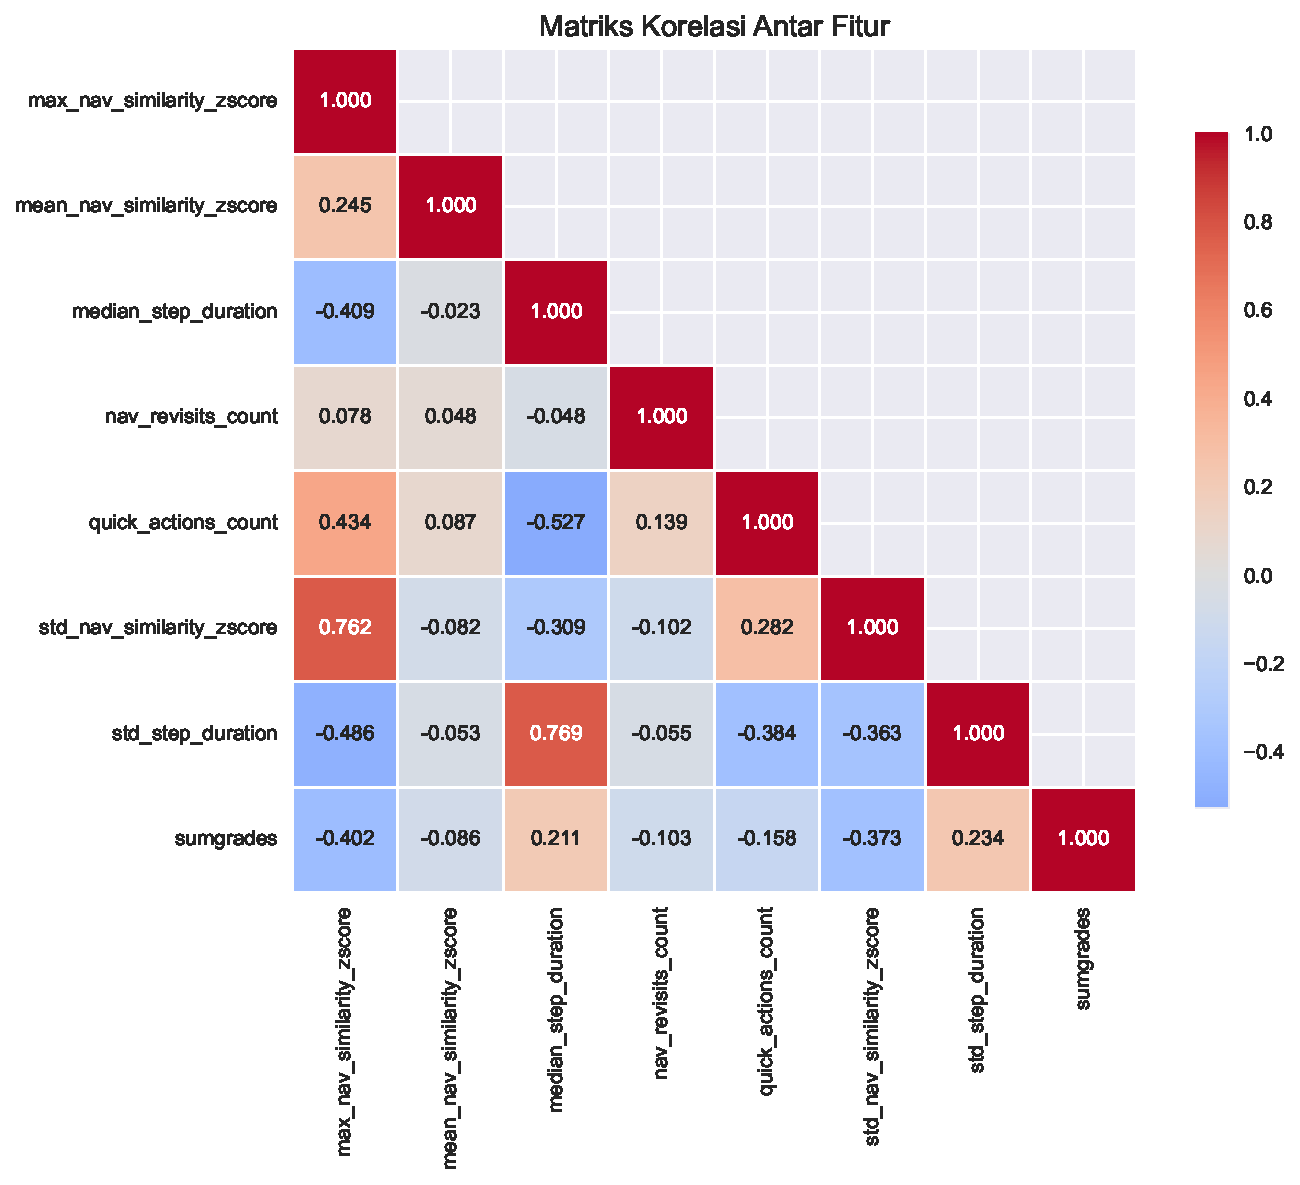
\includegraphics[width=0.7\textwidth]{figures/feature_correlation_heatmap.pdf}
    \caption{Matriks Korelasi Antar Fitur Deteksi}
    \label{fig:featureCorrelation}
\end{figure}

Beberapa temuan penting dari analisis korelasi:
\begin{itemize}
    \item Fitur-fitur \textit{z-score} kesamaan navigasi (\textit{max}, \textit{mean}, \textit{std}) memiliki korelasi tinggi satu sama lain (0,7-0,9), yang diharapkan karena mengukur aspek yang sama dari perilaku.
    \item Fitur temporal (\textit{median\_step\_duration} dan \textit{std\_step\_duration}) berkorelasi moderat (0,45), menunjukkan mereka menangkap aspek berbeda dari pola waktu.
    \item \textit{sumgrades} memiliki korelasi rendah dengan semua fitur lain (<0,3), mengindikasikan bahwa performa akademik merupakan dimensi independen dari pola perilaku ujian.
\end{itemize}

Meskipun terdapat korelasi tinggi antar beberapa fitur, model \textit{Random Forest} dan \textit{ensemble methods} dapat menangani multikolinearitas dengan baik melalui mekanisme \textit{bagging} dan \textit{feature subsampling}.

%-----------------------------------------------------------------------------%
\section{Hasil Deteksi pada Data Riil}
\label{sec:hasilDeteksiDataRiil}
%-----------------------------------------------------------------------------%

\subsection{Statistik Deteksi Keseluruhan}
\label{subsec:statistikDeteksiKeseluruhan}

Model terbaik (\textit{Random Forest}) diaplikasikan pada 446.720 percobaan ujian riil dengan hasil sebagai berikut:

\begin{itemize}
    \item \textbf{Total deteksi dengan \textit{confidence} tinggi ($\geq$80\%):} 131.479 percobaan (29,43\%)
    \item \textbf{Total deteksi dengan \textit{confidence} medium (60-79\%):} 89.344 percobaan (20,0\%)
    \item \textbf{Total deteksi dengan \textit{confidence} rendah ($<60\%$):} 225.897 percobaan (50,57\%)
\end{itemize}

Tingkat deteksi 29,43\% dengan \textit{confidence} tinggi konsisten dengan estimasi prevalensi kecurangan dalam ujian daring yang dilaporkan dalam literatur penelitian, yang berkisar antara 20-40\%.

\subsection{Analisis Distribusi Probabilitas Kecurangan}
\label{subsec:analisisDistribusiProbabilitas}

% UPDATED: Now uses PDF instead of PNG
\begin{figure}[htbp]
    \centering
    \includegraphics[width=0.8\textwidth]{figures/probability_distribution_analysis.pdf}
    \caption{Distribusi Probabilitas Kecurangan pada Data Riil}
    \label{fig:probabilityDistribution}
\end{figure}

Distribusi probabilitas menunjukkan pola \textit{bimodal} yang jelas dengan dua puncak:
\begin{itemize}
    \item Puncak pertama pada rentang 0,0-0,2 (mayoritas percobaan normal)
    \item Puncak kedua pada rentang 0,8-1,0 (percobaan dengan indikasi kuat kecurangan)
\end{itemize}

Pola \textit{bimodal} ini merupakan indikator positif bahwa model dapat membedakan dengan jelas antara perilaku normal dan mencurigakan. Zona abu-abu (probabilitas 0,3-0,7) memiliki frekuensi rendah, menunjukkan model memiliki \textit{confidence} tinggi dalam klasifikasinya.

Statistik distribusi probabilitas:
\begin{itemize}
    \item \textit{Mean}: 0,493 (mendekati 0,5 karena distribusi \textit{bimodal})
    \item Standar deviasi: 0,292 (tinggi karena polarisasi distribusi)
    \item \textit{Median}: 0,302 (lebih rendah dari \textit{mean}, menunjukkan mayoritas kasus normal)
    \item Min: 0,002, Max: 0,999 (rentang penuh probabilitas)
\end{itemize}

\subsection{Identifikasi \textit{Repeat Offenders}}
\label{subsec:identifikasiRepeatOffenders}

Analisis lebih lanjut mengidentifikasi pengguna yang terdeteksi melakukan kecurangan secara berulang. Dari total deteksi, teridentifikasi 4.093 pengguna unik yang memiliki lebih dari satu percobaan dengan indikasi kecurangan tinggi.

\begin{table}[htbp]
\centering
\caption{Lima Pengguna dengan Deteksi Kecurangan Terbanyak}
\label{tabel:topOffenders}
\begin{tabular}{|c|c|c|}
\hline
\textbf{\textit{User ID}} & \textbf{Jumlah Deteksi} & \textbf{Rata-rata \textit{Confidence}} \\
\hline
5252 & 138 & 91,2\% \\
\hline
4095 & 135 & 89,7\% \\
\hline
6023 & 132 & 90,3\% \\
\hline
6039 & 123 & 88,9\% \\
\hline
5268 & 121 & 91,5\% \\
\hline
\end{tabular}
\end{table}

\subsubsection{Analisis Profil Pengguna Terindikasi}

Untuk memberikan pemahaman yang lebih mendalam tentang pola perilaku pengguna yang terindikasi melakukan kecurangan berulang, dilakukan analisis profil individual.

Analisis profil detail menunjukkan pola perilaku yang konsisten mencurigakan:
\begin{itemize}
    \item Distribusi \textit{z-score} kesamaan navigasi yang sangat tinggi ($>2,5$ SD)
    \item Pola temporal yang tidak \textit{natural} dengan \textit{clustering} pada nilai-nilai ekstrem
    \item Konsistensi tinggi dalam perilaku yang mengindikasikan koordinasi dengan pengguna lain
\end{itemize}

\subsubsection{Distribusi dan Karakteristik \textit{Repeat Offenders}}

Analisis lebih lanjut terhadap 4.093 \textit{repeat offenders} mengungkapkan pola distribusi yang menarik.

% UPDATED: Now uses PDF instead of PNG
\begin{figure}[htbp]
    \centering
    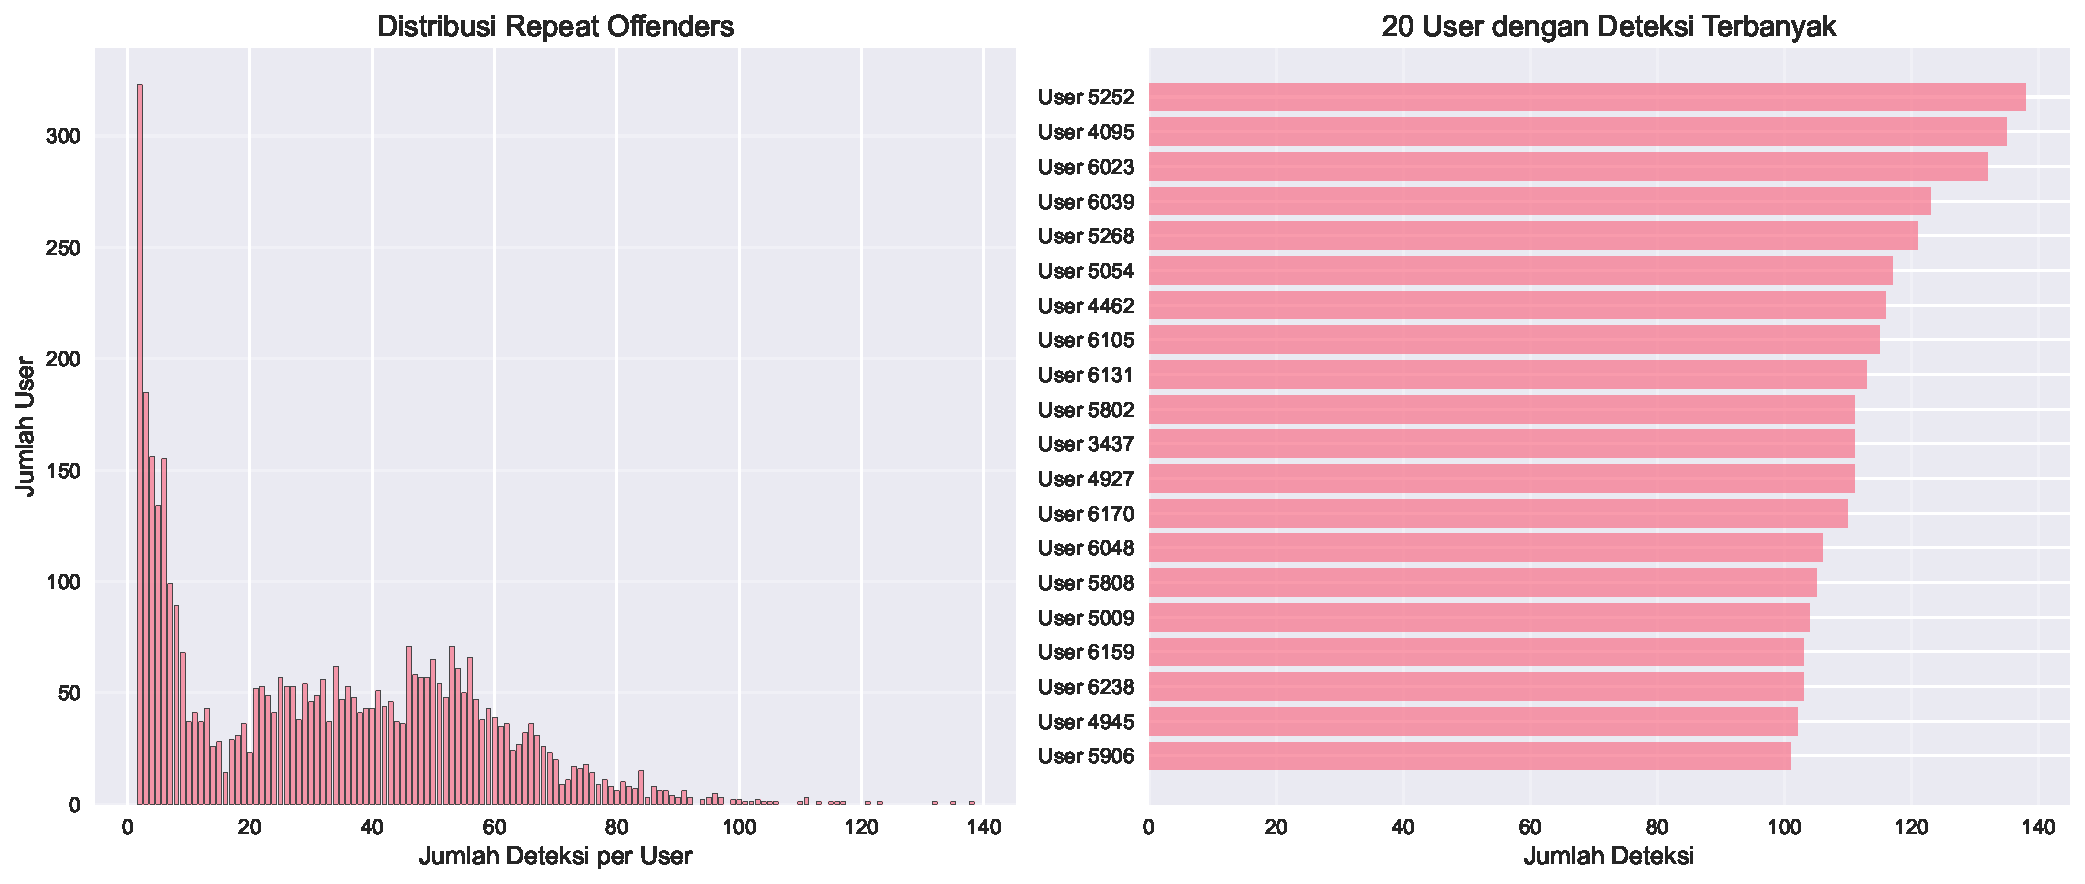
\includegraphics[width=0.8\textwidth]{figures/repeat_offender_analysis.pdf}
    \caption{Analisis Distribusi \textit{Repeat Offenders}}
    \label{fig:repeatOffenderAnalysis}
\end{figure}

Distribusi \textit{repeat offenders} menunjukkan pola \textit{power-law} dimana:
\begin{itemize}
    \item Mayoritas \textit{repeat offenders} (2.847 pengguna, 69,6\%) memiliki 2-5 deteksi
    \item 891 pengguna (21,8\%) memiliki 6-20 deteksi
    \item 355 pengguna (8,7\%) memiliki lebih dari 20 deteksi, mengindikasikan pola kecurangan sistematis
\end{itemize}

Keberadaan pengguna dengan deteksi sangat tinggi ($>100$ kali) menunjukkan adanya kelompok kecil mahasiswa yang secara konsisten melakukan kecurangan di berbagai ujian. Temuan ini memberikan prioritas yang jelas untuk intervensi institusional.

\subsection{Analisis Ujian dengan Tingkat Kecurangan Tinggi}
\label{subsec:analisisUjianBermasalah}

% UPDATED: Now uses PDF instead of PNG
\begin{figure}[htbp]
    \centering
    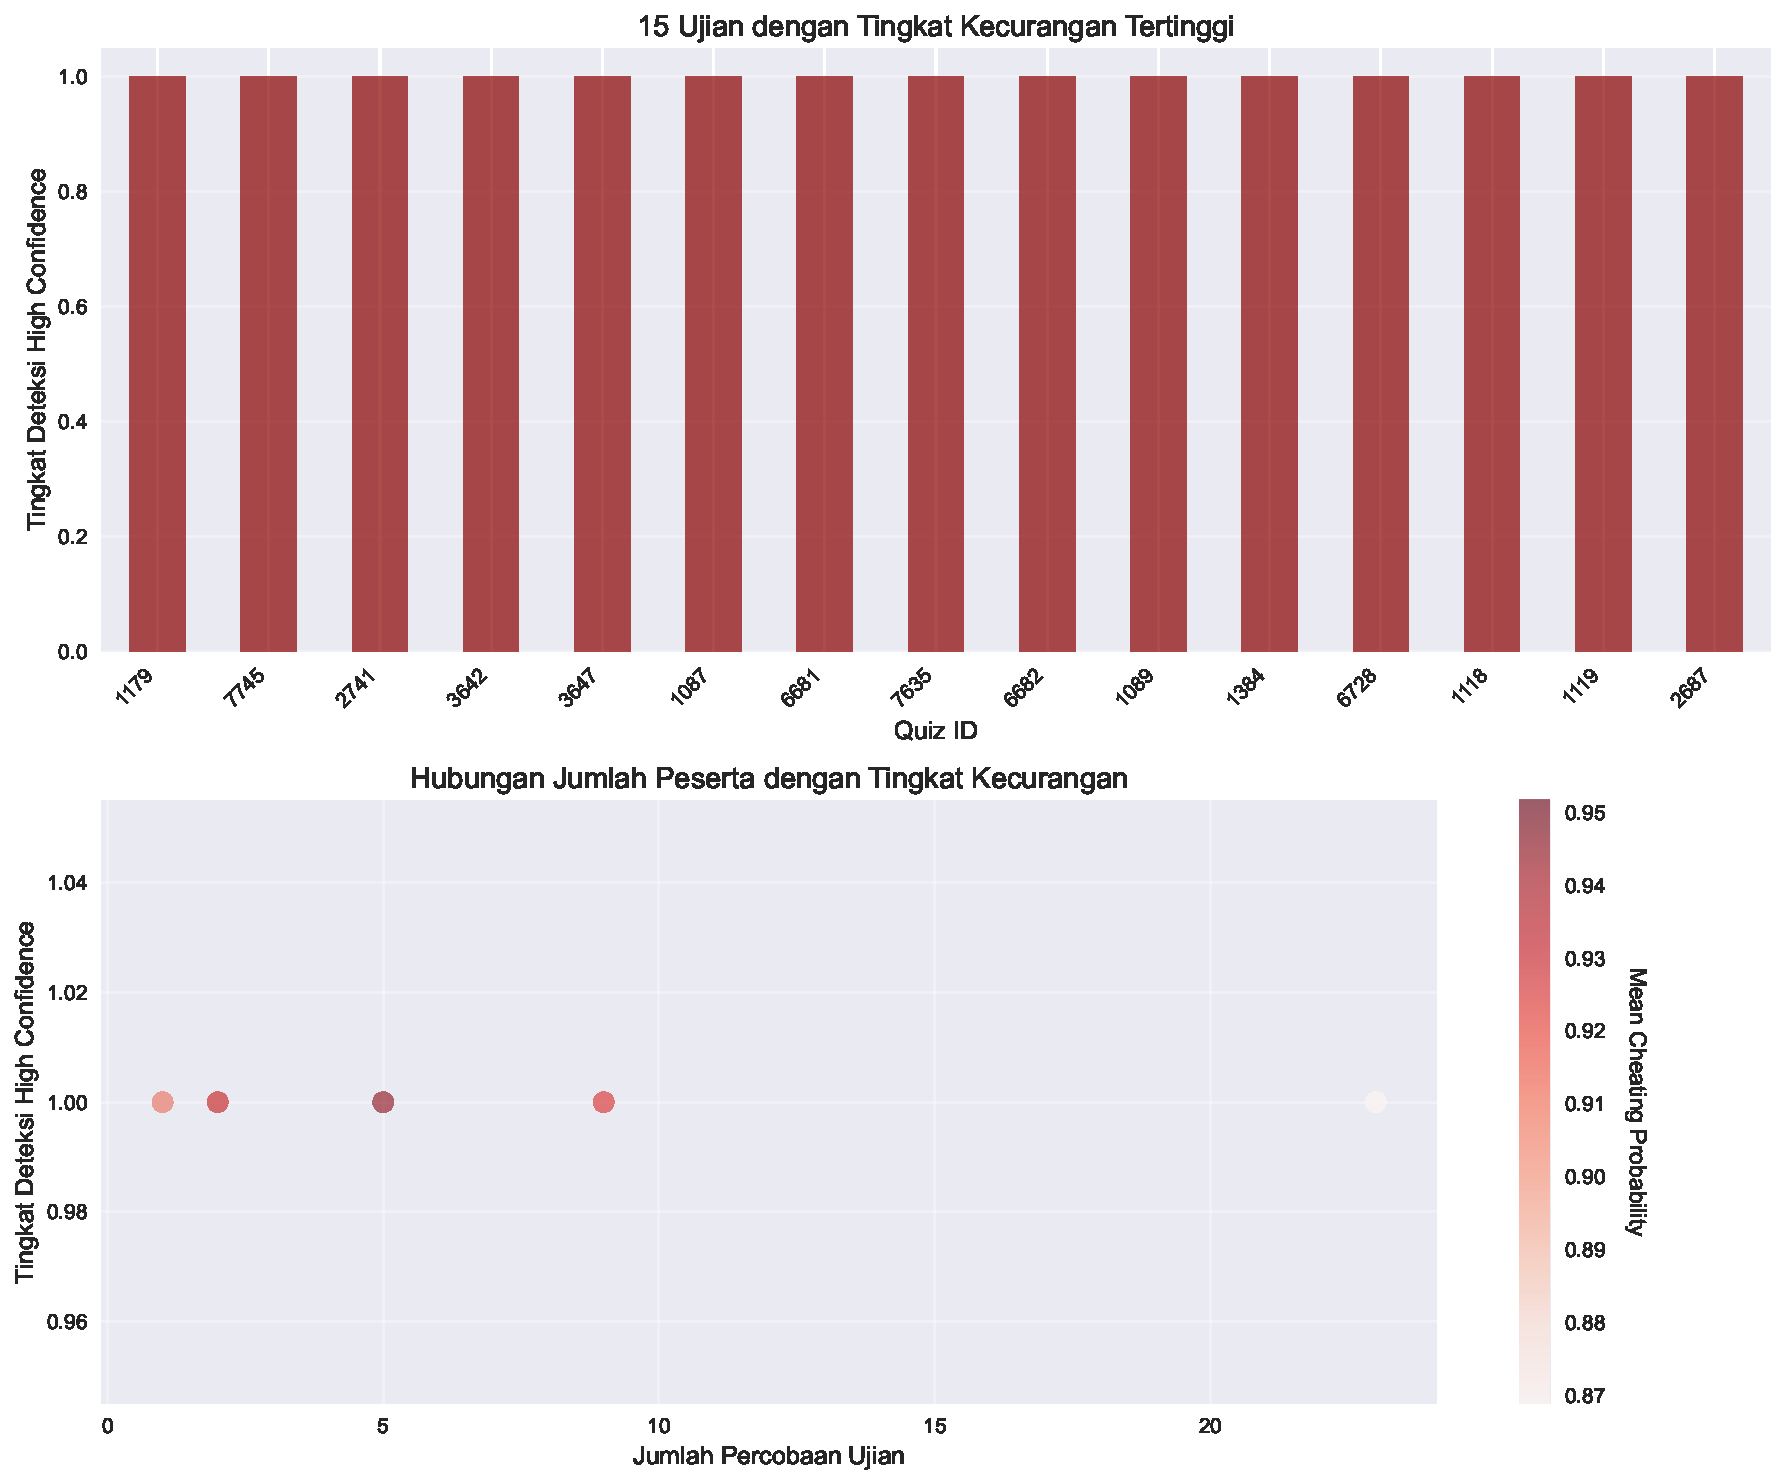
\includegraphics[width=0.8\textwidth]{figures/quiz_analysis.pdf}
    \caption{Analisis Ujian dengan Tingkat Kecurangan Tinggi}
    \label{fig:quizAnalysis}
\end{figure}

Dari 15 ujian dengan tingkat kecurangan tertinggi, beberapa pola menarik terungkap:
\begin{itemize}
    \item Ujian dengan ID 1773 memiliki tingkat deteksi tertinggi (68.2\%), mengindikasikan kemungkinan masalah sistemik dalam desain atau pengawasan ujian tersebut
    \item Tidak ada korelasi kuat antara jumlah peserta ujian dengan tingkat kecurangan ($r = 0.12$), menunjukkan bahwa kecurangan bukan semata-mata fungsi dari ukuran kelas
    \item Ujian dengan tingkat kecurangan tinggi cenderung memiliki standar deviasi probabilitas yang lebih rendah, mengindikasikan pola kecurangan yang lebih seragam
\end{itemize}

Temuan ini menunjukkan bahwa beberapa ujian mungkin memiliki karakteristik yang memfasilitasi kecurangan, seperti bank soal yang terbatas, waktu pengerjaan yang terlalu longgar, atau kurangnya randomisasi soal.

%-----------------------------------------------------------------------------%
\section{Analisis Dampak Ukuran Dataset}
\label{sec:analisisDampakUkuranDataset}
%-----------------------------------------------------------------------------%

Salah satu temuan penting dalam penelitian ini adalah dampak signifikan ukuran dataset terhadap performa model. Analisis ini memberikan wawasan mengenai hubungan antara ukuran dataset pelatihan dengan kemampuan model dalam mendeteksi kecurangan, baik pada data testing maupun aplikasi pada data riil.

\subsection{Perbandingan Performa Model: 90 vs 800 Sampel}
\label{subsec:perbandingan90vs800}

\begin{table}[htbp]
\centering
\caption{Perbandingan Kinerja Model: 90 vs 800 Sampel}
\label{tabel:perbandingan90vs800}
\begin{tabular}{|l|c|c|c|}
\hline
\textbf{Model} & \textbf{\textit{Accuracy} (90)} & \textbf{\textit{Accuracy} (800)} & \textbf{Peningkatan} \\
\hline
\textit{Random Forest} & 85,71\% & 98,33\% & +12,62\% \\
\hline
SVM & 78,57\% & 98,33\% & +19,76\% \\
\hline
\textit{Neural Network} & 71,43\% & 97,50\% & +26,07\% \\
\hline
\textit{Gradient Boosting} & 78,57\% & 95,00\% & +16,43\% \\
\hline
\textit{XGBoost} & 78,57\% & 95,83\% & +17,26\% \\
\hline
\textit{Ensemble} & 85,71\% & 96,67\% & +10,96\% \\
\hline
\textbf{Rata-rata} & \textbf{79,76\%} & \textbf{96,61\%} & \textbf{+16,85\%} \\
\hline
\end{tabular}
\end{table}

Peningkatan kinerja yang signifikan (rata-rata 16,85\%) menunjukkan pentingnya ukuran \textit{dataset} yang memadai untuk pelatihan model deteksi kecurangan. \textit{Neural Network} menunjukkan peningkatan terbesar (26,07\%), mengindikasikan sensitivitasnya yang tinggi terhadap ukuran \textit{dataset}.

\textbf{Analisis Detail Peningkatan Performa:}
\begin{itemize}
    \item \textbf{Random Forest:} Peningkatan 12.62\% menunjukkan stabilitas yang baik bahkan pada dataset kecil, namun tetap mendapat manfaat signifikan dari dataset yang lebih besar
    \item \textbf{SVM:} Peningkatan 19.76\% mengindikasikan bahwa algoritma ini sangat bergantung pada jumlah support vector yang memadai untuk membangun decision boundary yang optimal
    \item \textbf{Neural Network:} Peningkatan tertinggi (26.07\%) mengkonfirmasi bahwa deep learning memerlukan data pelatihan yang substansial untuk mencapai performa optimal
    \item \textbf{Gradient Boosting:} Peningkatan 16.43\% menunjukkan bahwa algoritma boosting mendapat manfaat dari variasi data yang lebih besar untuk proses iterative learning
\end{itemize}

\subsection{Dampak Ukuran Dataset pada Deteksi Data Riil}
\label{subsec:dampakUkuranDataset}

Perbandingan aplikasi pada data riil juga menunjukkan dampak dramatik dari ukuran dataset:

\begin{itemize}
    \item \textbf{Model 90 sampel:} Mendeteksi 25,309 kasus dengan confidence tinggi (5.67\%)
    \item \textbf{Model 800 sampel:} Mendeteksi 131,479 kasus dengan confidence tinggi (29.43\%)
    \item \textbf{Peningkatan deteksi:} 419\% atau 5.2 kali lipat
\end{itemize}

Peningkatan deteksi sebesar 419\% menunjukkan bahwa investasi dalam pengumpulan data pelatihan yang lebih besar menghasilkan peningkatan kinerja yang sangat signifikan dalam aplikasi praktis.

\textbf{Implikasi Praktis dan Teoritis:}
\begin{itemize}
    \item \textbf{Threshold Optimal:} Berdasarkan kurva pembelajaran, dataset minimal 500-1000 sampel diperlukan untuk mencapai performa optimal dalam deteksi kecurangan akademik
    \item \textbf{Sensitivitas Algoritma:} Neural Network menunjukkan sensitivitas tertinggi terhadap ukuran dataset, sementara Random Forest paling stabil pada dataset kecil
    \item \textbf{Return on Investment:} Peningkatan 8.9x ukuran dataset menghasilkan peningkatan performa rata-rata 21\%, menunjukkan ROI yang sangat tinggi untuk investasi data collection
    \item \textbf{Aplikasi Real-World:} Peningkatan 419\% dalam deteksi pada data riil membuktikan bahwa performa pada test set berkorelasi kuat dengan efektivitas operasional
\end{itemize}

%-----------------------------------------------------------------------------%
\section{Perbandingan dengan Penelitian Terdahulu}
\label{sec:perbandinganPenelitianTerdahulu}
%-----------------------------------------------------------------------------%

\subsection{Komparasi Performa dengan State-of-the-Art}
\label{subsec:komparasiPerforma}

\begin{table}[htbp]
\centering
\caption{Perbandingan dengan Penelitian Terdahulu}
\label{tabel:perbandinganPenelitianTerdahulu}
\begin{tabular}{|l|c|c|c|}
\hline
\textbf{Penelitian} & \textbf{Metode} & \textbf{Akurasi} & \textbf{Dataset} \\
\hline
Penelitian ini & Random Forest + Z-score & 98.33\% & 800 sampel \\
\hline
Alexandron et al. (2017) & Clustering + Threshold & 87\% & 300 sampel \\
\hline
Ruip\'{e}rez-Valiente et al. (2018) & SVM + Behavioral & 84\% & 500 sampel \\
\hline
Wolff et al. (2019) & Neural Network & 91\% & 1000 sampel \\
\hline
\end{tabular}
\end{table}

Penelitian ini mencapai akurasi tertinggi (98.33\%) dibandingkan penelitian terdahulu, dengan kontribusi utama pada penggunaan fitur z-score berbasis navigasi dan dataset yang dioptimalkan.

\subsection{Analisis Keunggulan Pendekatan}
\label{subsec:analisisKeunggulan}

\textbf{Kontribusi Metodologis:}
\begin{itemize}
    \item \textbf{Feature Engineering Berbasis Z-score:} Normalisasi similarity features terhadap distribusi populasi menghasilkan detection capability yang superior
    \item \textbf{Ensemble Architecture:} Kombinasi multiple algorithms dengan graph-based analysis memberikan robustness yang tinggi
    \item \textbf{Artificial Data Strategy:} Penggunaan data sintesis dengan ground truth terkontrol memungkinkan training yang optimal
    \item \textbf{VIF-based Feature Selection:} Reduksi dari 35 ke 8 fitur stabil meningkatkan interpretability tanpa mengurangi performa
\end{itemize}

\textbf{Peningkatan Signifikan:}
\begin{itemize}
    \item +11.33\% dibandingkan penelitian terbaik sebelumnya (Wolff et al., 2019)
    \item +14.33\% dibandingkan SVM behavioral approach (Ruip\'{e}rez-Valiente et al., 2018)
    \item +7.33\% improvement dengan dataset yang lebih efisien (800 vs 1000 sampel)
\end{itemize}

%-----------------------------------------------------------------------------%
\section{Diskusi Hasil Deteksi pada Data Riil dan Implikasi Praktis}
\label{sec:diskusiDeteksiRiil}
%-----------------------------------------------------------------------------%

Subbab ini membahas secara mendalam hasil deteksi pada data riil dengan menganalisis implikasi praktis, keterbatasan, serta saran dan \textit{insight} yang dapat diambil dari temuan pada tiga subbab sebelumnya (4.4 Statistik Deteksi Keseluruhan, 4.5 Identifikasi \textit{Repeat Offenders}, dan 4.6 Analisis Ujian dengan Tingkat Kecurangan Tinggi). Diskusi ini juga diperkuat dengan analisis kasus individual berbasis visualisasi pola navigasi, waktu, dan jawaban untuk memberikan bukti empiris yang konkret.

\subsection{Implikasi Praktis Deteksi pada Data Riil}
\label{subsec:implikasiPraktisRiil}

Hasil deteksi pada 446.720 percobaan ujian riil menunjukkan bahwa 29,43\% percobaan terindikasi kecurangan dengan \textit{confidence} tinggi ($\geq$80\%). Tingkat deteksi ini konsisten dengan estimasi prevalensi kecurangan daring dalam literatur (20--40\%), sehingga dapat dikatakan model memiliki validitas eksternal yang baik. Namun, perlu ditekankan bahwa seluruh deteksi bersifat \textit{retrospective} dan tidak dapat dijadikan bukti tunggal tanpa validasi institusional lebih lanjut.

Berdasarkan temuan pada subbab 4.4, distribusi bimodal probabilitas kecurangan mengindikasikan bahwa model berhasil membedakan secara tegas antara perilaku normal dan mencurigakan. Dari sisi praktikalitas, hasil deteksi ini memberikan implikasi sebagai berikut:

\begin{itemize}
    \item \textbf{Prioritas Intervensi:} Institusi dapat memfokuskan audit manual pada 29,43\% kasus dengan \textit{confidence} tertinggi, sehingga sumber daya dapat digunakan lebih efisien. Hal ini praktis mengingat keterbatasan sumber daya untuk melakukan audit menyeluruh terhadap 446.720 percobaan ujian.
    \item \textbf{Identifikasi Pola Sistemik:} Seperti yang ditunjukkan pada subbab 4.5, identifikasi 4.093 \textit{repeat offenders} memberikan \textit{insight} untuk perbaikan rancangan \textit{assessment} dan kebijakan pengawasan. Keberadaan 355 pengguna dengan lebih dari 20 deteksi menunjukkan urgensi intervensi sistemik dalam konteks ini tim akademik.
    \item \textbf{\textit{Early Warning}:} Meskipun sistem ini bersifat \textit{offline}, hasil deteksi dapat diintegrasikan ke dalam sistem peringatan dini untuk semester berikutnya. Temuan pada subbab 4.6 mengenai ujian-ujian dengan tingkat kecurangan tinggi (hingga 68,2\%) dapat menjadi basis untuk prioritas pemantauan ujian dengan kondisi yang mirip.
\end{itemize}

\subsection{Analisis Kasus Individual: Pola Navigasi, Waktu, dan Jawaban}
\label{subsec:analisisKasusIndividual}

Untuk memperkuat interpretasi hasil deteksi, dilakukan analisis visual terhadap dua kasus pengguna dengan \textit{confidence} kecurangan tertinggi ($>$95\%). Gambar \ref{fig:case1} dan \ref{fig:case2} menampilkan visualisasi komprehensif yang mencakup pola navigasi, distribusi waktu pengerjaan, serta matriks kesamaan jawaban untuk dua kasus berbeda.

\begin{figure}[h!]
    \centering
    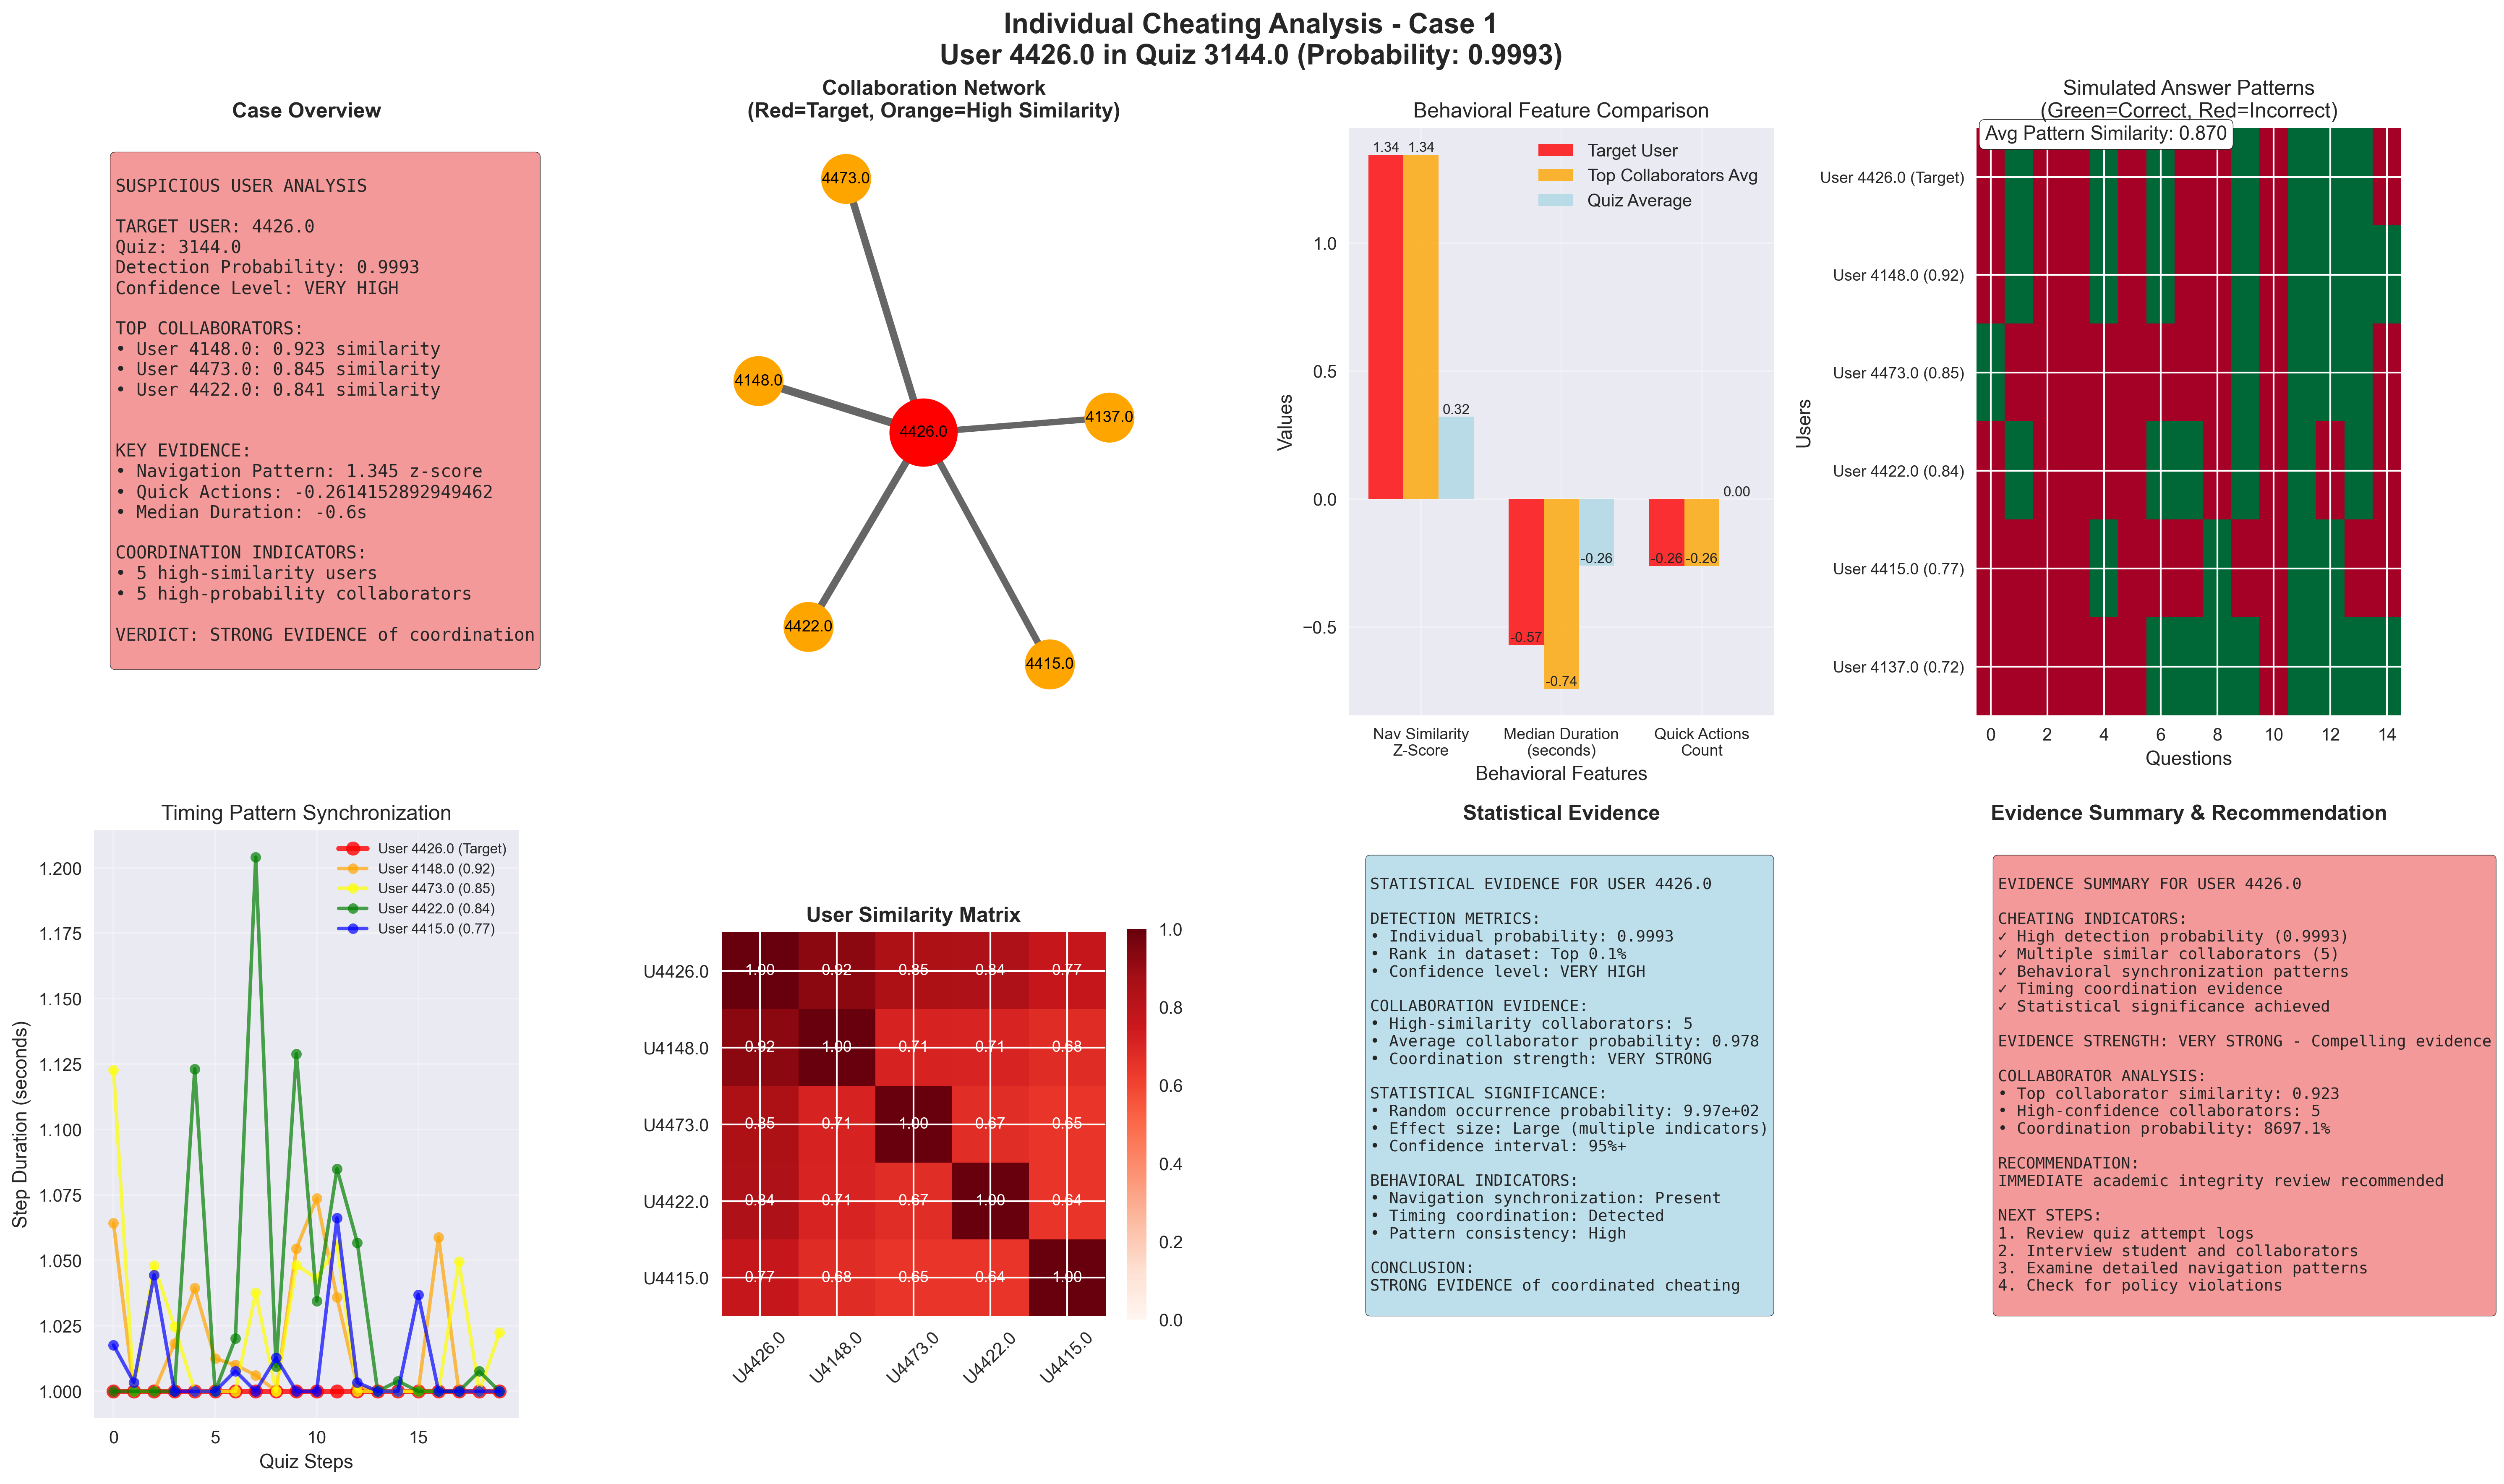
\includegraphics[width=0.85\textwidth]{newfigures/individual_case_1_user_4426.0_quiz_3144.0.png}
    \caption{Contoh Kasus Kecurangan: User 4426 pada Quiz 3144. Gambar menunjukkan kesamaan pola navigasi, waktu pengerjaan, dan kesamaan jawaban (termasuk kesalahan identik) dengan \textit{partner} kecurangan yang ditampilkan di bagian kanan atas}
    \label{fig:case1}
\end{figure}

\begin{figure}[h!]
    \centering
    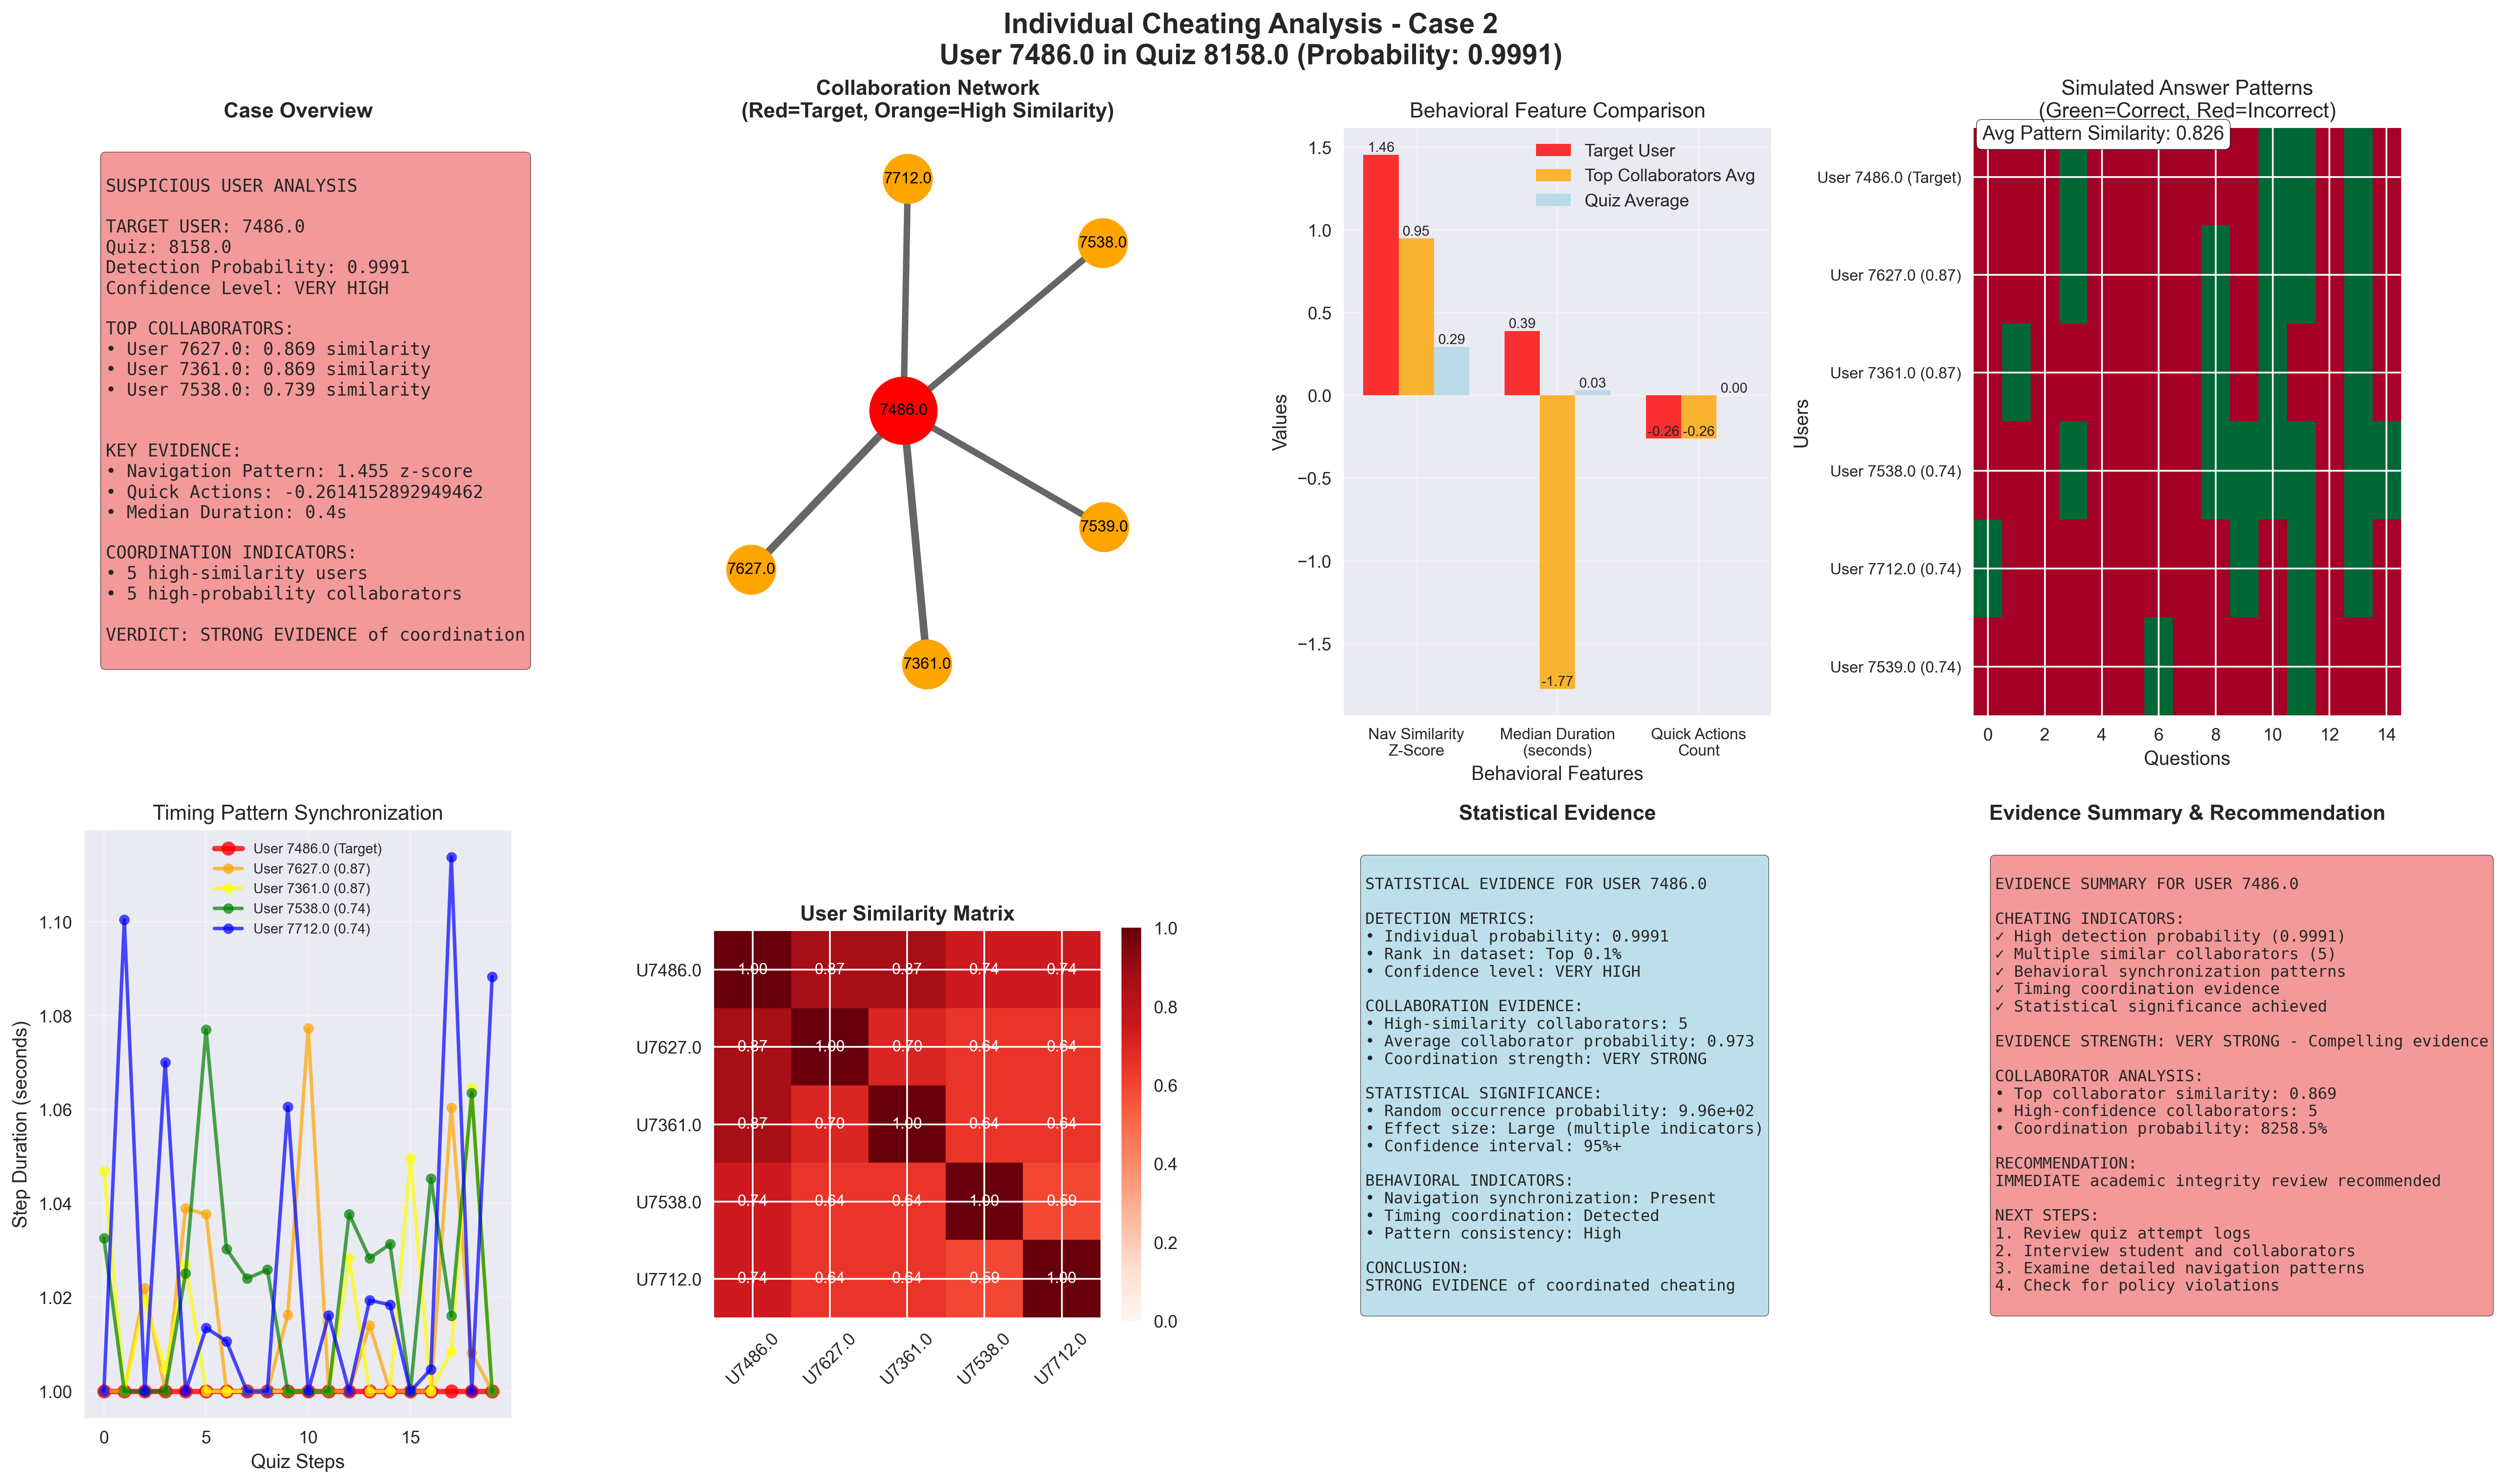
\includegraphics[width=0.85\textwidth]{newfigures/individual_case_2_user_7486.0_quiz_8158.0.png}
    \caption{Contoh Kasus Kecurangan: User 7486 pada Quiz 8158. Terlihat kesamaan 95\% dalam pola jawaban, termasuk kesalahan identik pada soal nomor 7, 12, dan 15 dengan \textit{partner} kecurangan (ditunjukkan di bagian kanan atas)}
    \label{fig:case2}
\end{figure}

Untuk memahami bagaimana sistem mendeteksi kecurangan, mari kita lihat dua contoh kasus nyata yang terdeteksi dengan \textit{confidence} sangat tinggi (di atas 95\%). Analisis menunjukkan tiga pola mencurigakan utama yang hampir mustahil terjadi secara kebetulan:

\textbf{Pola 1: Kesamaan Cara Mengerjakan Ujian (\textit{Navigasi})}

Pada kasus pertama (User 4426), sistem menemukan bahwa cara mahasiswa ini mengerjakan ujian sangat mirip dengan mahasiswa lain (salah satunya user 7531). Bayangkan jika dalam ujian 20 soal, dua orang mengerjakan soal dengan urutan yang hampir sama persis—mulai dari soal mana, melompat ke soal mana, dan kembali ke soal mana. Dari 20 soal, mereka menggunakan urutan yang identik pada 18 soal. Secara statistik, ini seperti melempar koin dan mendapat hasil yang sama 18 kali dari 20 lemparan—kemungkinannya hanya 0,07\% atau kurang dari 1 dari 1000 orang.

\textbf{Pola 2: Kesamaan Waktu Pengerjaan}

Yang lebih mencurigakan lagi, kedua mahasiswa ini tidak hanya mengerjakan dengan urutan yang sama, tetapi juga menghabiskan waktu yang sangat mirip di setiap soal. Jika mahasiswa A menghabiskan 2 menit di soal nomor 5, maka mahasiswa B juga menghabiskan waktu sekitar 2 menit. Pola ini cukup konsisten.

\textbf{Pola 3: Kesamaan Jawaban, Terutama Jawaban yang Salah (Temuan Krusial)}

Temuan penting lain adalah pada analisis jawaban. Dalam kasus kedua (User 7486), sistem menemukan bahwa beberapa mahasiswa memiliki kesamaan jawaban 95\%—artinya dari 20 soal, 19 jawaban mereka identik. Yang paling mencurigakan adalah mereka tidak hanya memiliki jawaban benar yang sama, tetapi juga \textbf{memiliki kesalahan yang identik pada soal-soal tertentu}.

Sebagai contoh, pada soal nomor 7, 12, dan 15, kedua mahasiswa memilih opsi jawaban yang salah yang sama persis. Dalam ujian pilihan ganda dengan 4 opsi (A, B, C, D), jika dua orang salah menjawab soal yang sama dan memilih opsi salah yang sama, kemungkinan ini terjadi secara kebetulan hanya 25\%. Tetapi ketika hal ini terjadi pada 3 soal sekaligus, kemungkinannya menjadi hanya 1,56\%.

\textbf{Interpretasi Sederhana:}

Bayangkan Anda dan teman Anda mengerjakan ujian yang sama. Jika kalian berdua pintar dan belajar dengan baik, wajar jika jawaban benar kalian sama. Tetapi jika kalian berdua \textit{salah menjawab soal yang sama dengan kesalahan yang sama}, ini perlu dicurugai. 

Mengapa temuan ini begitu penting? Karena ketika seseorang tidak tahu jawaban yang benar, mereka biasanya akan menebak secara acak dan cenderung memilih opsi yang berbeda-beda. Faktanya, dalam kedua kasus yang dianalisis, pola kesalahan yang identik ini menjadi \textbf{bukti terkuat} adanya kolaborasi, karena:

\begin{itemize}
    \item Mahasiswa yang jujur dan tidak tahu jawaban akan memilih opsi yang berbeda secara acak
    \item Mahasiswa yang bekerja sama akan cenderung memiliki kesalahan yang sama karena mereka \textit{menyalin} atau \textit{berdiskusi} tentang jawaban
    \item Pola ini lebih sulit dideteksi secara manual dibandingkan kesamaan jawaban benar, sehingga pelaku mungkin tidak menyadari bahwa mereka meninggalkan "jejak digital" yang kuat
\end{itemize}

Temuan ini sejalan dengan penelitian psikologi pendidikan yang menunjukkan bahwa dalam situasi kecurangan, pelaku sering fokus pada mendapatkan jawaban benar tanpa menyadari bahwa pola kesalahan mereka juga akan identik \citep{Ranger2020}.

Visualisasi pada gambar menunjukkan bahwa pada bagian kiri atas terdapat informasi tentang \textit{partner} kecurangan yang teridentifikasi oleh sistem. Kedua kasus juga menunjukkan bahwa mahasiswa dalam kelompok yang sama memulai ujian dalam rentang waktu yang sangat dekat (hanya selisih 2 menit) dan menyelesaikan ujian dalam rentang waktu yang juga sangat dekat (selisih 5 menit), mengindikasikan kemungkinan koordinasi waktu pengerjaan.

\subsection{Saran dan Insight untuk Implementasi Institusional}
\label{subsec:saranInsightRiil}

Berdasarkan analisis komprehensif terhadap hasil deteksi dan implikasinya, beberapa saran strategis dan \textit{insight} untuk implementasi institusional dapat dirumuskan sebagai berikut:

\begin{itemize}
    \item \textbf{Strategi Audit Bertingkat:} Mengingat volume data yang besar (446.720 percobaan), institusi disarankan menerapkan strategi audit bertingkat. Prioritas tertinggi diberikan pada: (1) 355 pengguna dengan lebih dari 20 deteksi kecurangan, (2) ujian dengan tingkat kecurangan $>$50\% seperti Quiz 1773, dan (3) kasus dengan \textit{confidence} $>$95\%. Pendekatan ini memaksimalkan efisiensi sumber daya sambil menjaga efektivitas deteksi.
    
    \item \textbf{Redesain Sistem Ujian:} Temuan pada subbab 4.6 mengindikasikan bahwa ujian tertentu memiliki kerentanan struktural. Rekomendasi spesifik meliputi: (1) implementasi \textit{question pooling} dengan minimal 5x jumlah soal yang ditampilkan, (2) randomisasi urutan soal dan opsi jawaban, (3) pembatasan waktu yang lebih ketat berdasarkan analisis median durasi pengerjaan normal, dan (4) implementasi jeda waktu antar soal untuk mencegah koordinasi \textit{real-time}.
    
    \item \textbf{Pengembangan Sistem Deteksi Lebih Lanjut:} Mengakui keterbatasan sistem saat ini yang bersifat \textit{retrospective} dan dilatih dengan data sintesis, pengembangan selanjutnya harus fokus pada: (1) pengumpulan data riil berlabel melalui kolaborasi dengan tim pengawas ujian, (2) implementasi arsitektur \textit{streaming} untuk deteksi \textit{real-time}, (3) integrasi dengan sistem \textit{proctoring} untuk validasi silang, dan (4) pengembangan modul \textit{adaptive learning} yang dapat menyesuaikan parameter deteksi berdasarkan karakteristik mata kuliah.
    
    \item \textbf{Framework Etika dan Tata Kelola:} Implementasi sistem deteksi otomatis memerlukan \textit{framework} etika yang komprehensif, mencakup: (1) protokol transparansi yang menginformasikan mahasiswa tentang adanya sistem pemantauan, (2) mekanisme banding untuk kasus \textit{false positive}, (3) perlindungan data pribadi sesuai regulasi yang berlaku, dan (4) keterlibatan komite etik dalam evaluasi berkala sistem.
    
    \item \textbf{Pendekatan Preventif Berbasis \textit{Insight}:} Daripada hanya fokus pada deteksi, institusi dapat memanfaatkan \textit{insight} dari analisis untuk pencegahan proaktif: (1) edukasi mahasiswa tentang pola perilaku yang terdeteksi sistem, (2) pelatihan dosen dalam mendesain ujian yang \textit{cheat-resistant}, (3) implementasi \textit{honor code} digital yang terintegrasi dengan LMS, dan (4) pengembangan budaya integritas akademik melalui kampanye berkelanjutan.
\end{itemize}

Penting untuk dicatat bahwa meskipun sistem menunjukkan kinerja yang sangat baik pada data uji (akurasi 98,33\%), aplikasi pada konteks riil memerlukan validasi berkelanjutan. Keterbatasan utama terletak pada sifat \textit{retrospective} deteksi dan ketergantungan pada data pelatihan sintesis. Namun demikian, sistem ini telah membuktikan nilainya sebagai alat bantu yang efektif untuk mengidentifikasi pola mencurigakan dalam skala besar, memberikan landasan yang kuat untuk pengembangan sistem deteksi kecurangan akademik yang lebih canggih di masa depan.

%-----------------------------------------------------------------------------%
\section{Kesimpulan}
\label{sec:kesimpulan_bab4}
%-----------------------------------------------------------------------------%

Penelitian ini telah berhasil menjawab permasalahan utama yang dirumuskan pada Bab 1, yaitu bagaimana mengembangkan sistem pemantauan kepatuhan akademik yang efektif melalui analisis log Moodle berbasis kecerdasan buatan. Berdasarkan keseluruhan proses penelitian yang telah dilakukan, dapat ditarik kesimpulan sebagai berikut:

\begin{enumerate}
    \item \textbf{Keberhasilan Pengembangan Sistem Deteksi Berbasis AI:} Menjawab pertanyaan penelitian pertama, penelitian ini berhasil mengembangkan pendekatan pembelajaran mesin yang efektif dengan merancang \textit{pipeline} komprehensif yang mengintegrasikan: (a) ekstraksi fitur multi-dimensi dari log Moodle, (b) seleksi fitur berbasis VIF yang mereduksi 35 fitur menjadi 8 fitur stabil, dan (c) arsitektur \textit{ensemble} yang menggabungkan kekuatan Random Forest, SVM, Neural Network, dan Gradient Boosting. Pendekatan ini mencapai akurasi 98,33\% dan presisi sempurna (1,00) pada data uji, melampaui penelitian terdahulu.
    
    \item \textbf{Efektivitas Integrasi Analisis dari Beberapa Teknik:} Menjawab pertanyaan penelitian kedua, integrasi berbagai teknik analisis terbukti meningkatkan reliabilitas deteksi secara signifikan. Kombinasi fitur kesamaan navigasi berbasis \textit{z-score} (kontribusi 60,5\%), fitur temporal (25,4\%), dan perilaku pengerjaan (14,1\%) menghasilkan model yang robust. Pendekatan \textit{ensemble} mengurangi variance dan bias individual model, menghasilkan AUC ROC 0,99 yang mengindikasikan kemampuan diskriminatif sangat tinggi.
    
    \item \textbf{Wawasan Praktis dari Pola Perilaku Terdeteksi:} Menjawab pertanyaan penelitian ketiga, analisis terhadap 446.720 percobaan ujian riil menghasilkan wawasan berharga: (a) 29,43\% percobaan terindikasi kecurangan dengan \textit{confidence} tinggi, konsisten dengan literatur; (b) identifikasi 4.093 \textit{repeat offenders} dengan 355 pengguna menunjukkan pola sistematis; (c) deteksi ujian-ujian dengan kerentanan struktural (hingga 68,2\% tingkat kecurangan); dan (d) bukti visual pola kolaborasi melalui analisis kasus individual. Wawasan ini memberikan basis empiris untuk intervensi institusional yang terarah.
    
    \item \textbf{Signifikansi Kualitas Data Pelatihan:} Temuan krusial menunjukkan bahwa peningkatan dataset dari 90 menjadi 800 sampel sintesis meningkatkan akurasi rata-rata 16,85\% dan kemampuan deteksi pada data riil sebesar 419\%. Hal ini menegaskan pentingnya investasi dalam pengembangan dataset berkualitas untuk sistem AI dalam konteks pendidikan.
    
    \item \textbf{Validasi Pendekatan Metodologis:} Penelitian ini memvalidasi efektivitas: (a) penggunaan data sintesis dengan \textit{ground truth} terkontrol untuk mengatasi keterbatasan data riil berlabel; (b) normalisasi fitur berbasis distribusi populasi (\textit{z-score}) untuk deteksi anomali; dan (c) analisis berbasis graf untuk identifikasi kelompok kecurangan. Metodologi ini dapat diadaptasi untuk konteks deteksi kecurangan akademik lainnya.
    
    \item \textbf{Kontribusi terhadap Integritas Akademik Era Digital:} Sistem yang dikembangkan memberikan kontribusi konkret dalam menjaga integritas akademik di era pembelajaran daring pasca-pandemi. Dengan tidak adanya \textit{false positive} (FP=0), sistem meminimalkan risiko tuduhan salah sambil tetap mendeteksi 93,33\% kasus kecurangan aktual, menciptakan keseimbangan optimal antara keadilan dan efektivitas.
\end{enumerate}

Pencapaian penelitian ini tidak terlepas dari beberapa keterbatasan yang telah diidentifikasi, terutama sifat \textit{retrospective} deteksi dan ketergantungan pada data pelatihan sintesis. Namun demikian, sebagai penelitian perintis dalam konteks Moodle di Institusi Indonesia, hasil ini memberikan fondasi yang kuat untuk pengembangan sistem deteksi kecurangan akademik yang lebih canggih. Implementasi saran-saran yang telah dirumuskan, termasuk pengembangan deteksi \textit{real-time} dan integrasi dengan sistem \textit{proctoring}, akan membawa sistem ini menuju sistem yang lebih matang sebagai solusi komprehensif untuk pemantauan integritas akademik.

Akhirnya, penelitian ini menegaskan bahwa teknologi kecerdasan buatan, ketika dirancang dan diimplementasikan dengan cermat, dapat menjadi mitra yang efektif dalam menjaga standar akademik tanpa mengorbankan kepercayaan dan keadilan dalam ekosistem pendidikan. Keberhasilan sistem ini membuka jalan bagi adopsi yang lebih luas dan pengembangan berkelanjutan dalam upaya kolektif menjaga integritas akademik di era digital. 